\ot{Innledningen har fått mange kommentarer som ikke er inkludert enda? Lite fokus. Uklar norsk. Spesifikt: Hvem mener. Skriver. Hevder.}\ot{Det er her det er viktig med tittel. Hvor vil dere? Er multimorbiditet sentralt?} Med stadig økende levealder, overlevelsesrate og flere behandlingsmetoder øker medisin-og sykdomsbildet for eldre. \ot{Hva er et økende bilde? Et medisinbilde? Dette er kommentert før} Rundt to tredeler av alle pasienter over 65 år i Norge er multimorbide \citep{multimorbidity_trend}. Multimorbiditet forekommer i andre aldersgrupper, men er klart overrepresentert i geriatrien. Denne pasientgruppen trenger kontinuerlig oppfølging og behandling, noe som gjør dem de mest sårbare når det kommer til kontinuitet og koordinering i helsetjenesten.

I dag søkes det IKT-løsninger som primært kan deles inn i to områder. \citep{innovathon_helsit} \ot{Det må finnes bedre kilder å referere!}
\begin{itemize}
    \item Løsninger som kan bli brukt for å samle anonymisert data om personer med multimorbid diagnose fra mange ulike register.
    \item Løsning for å analysere data for å utvikle og validere kunnskap om optimal behandling og sammensetting av tjenester for multimorbide personer.
\end{itemize}
Motivasjonen bak å utvikle et system\ot{Hvilket system?} var å kunne delvis eller komplett dekke begge behov. Det er ofte flere institusjoner involvert i behandlingsprosessen av en multimorbid pasient. Dette kan føre til ytterligere utfordringer siden pasienten, klinisk personale og helsetjenesten fort mister oversikten over behandlingsprosessen. Hvis vårt system kunne holde oversikten samt levere analysert kunnskap ville vi kunne dekke begge behovene. Vi ønsket å kunne utvikle indikatorer som hjelper en klinisk farmasøyt i hverdagen ved legemiddegjennomgang av en pasient. Dette innebærer å identifisere optimale tiltak som har potensialet for forbedringer og forenkling. Potensielle gevinster et slikt system kan bringe er knyttet til reduseringer av kostnader, økt læringsutbytte og økt verdi og nytte av informasjon registrert av helsepersonell. Med redusering av kostnader mener vi at systemet kan potensielt redusere reinnleggelser samt redusere tidsbruk. Ved å øke læringsutbyttet kan en klinisk farmasøyt ta med seg tilegnet kunnskap videre, som kan forbedre prosessen og resultatet. Verdi- og nytteøkning av informasjon kan bidra til informasjonsgrunnlag av høy kvalitet\ot{betyr hva?}. Dette \ot{nytteøkning?} kan igjen brukes i utviklingen av mer presis teknologi for monitorering og beslutningsstøtte i fremtiden.\ot{For mange pronomen som ikke viser til noe som passer setningsstruktur...}

\section{Motivasjon}
\subsection{Multimorbide pasienter - en behandlingsbyrde?}
Kronisk sykdom er vår tids store epidemi\ot{floskel}, men strategiene vi\ot{hvem} har utviklet for å håndtere det har skapt en økende byrde for pasientene. Pasienter med multimorbiditet har en \ot{norsk?} og selvhåndtering av egne tilstander, deltagelse i avtaler og møter med helsetjenesten samt håndtering av legemiddelregimer.\citep{min_disruptie_medicine} Pasienter opplever også en byrde ved at de erfarer fragmentering og dårlig koordinering av omsorg. Dette er ofte et resultat av pasienter får behandling av ulike helseinstitusjoner, som legger vekt på viktigheten av egne retningslinjer. Kommunikasjon mellom de forskjellige institusjonene er ofte suboptimal, noe som innvirker negativt på pasientutfallet. \citep{GPS_perspective_multimor} Slike behandlingsbyrder reduserer pasientens kapasitet til samarbeid om deres egen helse.

Hvorfor oppfattes multimorbiditet som en epidemi og hva vet vi om behandlingen av multisyke\ot{multimorbid=multisyk}? Det vi vet er at det finnes faktorer som gir multimorbide redusert effekt. Dette kan enten være at pasienten bare tar halvparten av legemidlene de skal ta, eller at fastlegen bare delvis følger retningslinjene. Et utfall av dette er utilsiktede hendelser som kommer av legemiddelrelaterte problemer. Om lag 7\% av innleggelser på sykehus kommer av legemiddelhendelser og er da en av de hyppigste innleggelsesårsakene. I tillegg til 1300 dødsfall i året er det et langt høyere antall skader. \citep{anders_grimsmo} Norske tall anslår 15 500 legemiddelskader hvert år, hvorav 50\% kan forebygges \citep{kvalitetogprioritering_multisyke}. Dette er skader hvorav noen er varige, for eksempel gjennombrudd av nye sykdommer som diabetes, Parkinson, hjertesvikt med mer\citep{anders_grimsmo}\todo{Finn mer presis kilde - spør}.
Majoriteten av utilsiktede legemiddelhendelser forekommmer hos multimorbide. Utilsiktede legemiddelhendelser kan få store følger samt redusere livskvaliteten for mange. Videre er multimorbide den største pasientgruppen både i antall og i risiko med henhold til reinleggelser. Det er derfor behov for et bedre kunnskapsgrunnlag for å øke kvaliteten og sikkerheten i diagnostikk og behandlingen av denne pasientgruppen. For å kunne møte disse behovene er det flere utfordringer knyttet multimorbiditet og polyfarmasi. Det er allerede satt i gang tiltak\ot{av hvem?} som kan bidra til riktigere legemiddelbruk, hvor legemiddelsamstemming og legemiddelgjennomgang er to av tre. Det finnes også utfordringer i volumet av retningslinjer brukes\ot{norsk?}, utilgjengelighet av retningslinjer, samt retningslinjer som fører til overdiagnostikk og overbehandling av pasienter.
\subsection{Legemiddelkjeden}
Legemiddelkjeden eller ofte kalt legemiddelsløyfen, er prosessene som inngår fra legen ordinerer et medikament, til bestilling, effektuering, leveranse og administrering av legemidler. Her er formålet å vise hvilke aktører som gjør hva i en slik prosesskjede. Figur \ref{legemiddelkjede} viser hvordan legemiddelkjeden typisk ser ut ved sykehus. 
\begin{figure}[!h]\ot{skill mellom helsevesenets, pasientens, legemiddelintervensjons - legmiddelkjede}
\centering
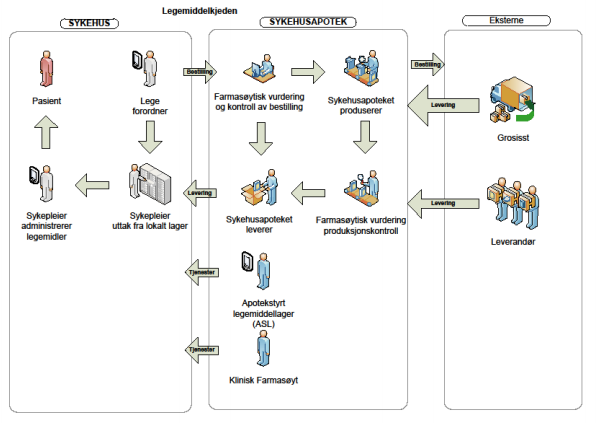
\includegraphics[width=140mm]{images/legemiddelkjede.PNG}
\caption{Legemiddelkjede ved sykehus(gjengitt fra \citep{Legemiddelberedskap_sykehusapotekene})}
\label{legemiddelkjede}
\end{figure}


\section{Problemområde}
\subsection{Samstemming av legemiddellister}
Det finnes ikke i dag en ''sann''  liste over hva pasienter bruker av medikamenter. Pasienters legemiddelbruk er ikke under samlet kontroll. Derimot har ulike institusjoner sine egne lister over hvilke medikamenter pasienter bruker, for eksempel i fastlegens EPJ, i pleie og omsorgstjenesten, sykehusets EPJ og i apotekene. Dette gir rom for feil og mye manuelt arbeid, da beskjeder om endring i legemiddelbruk ofte er i fritekstformat. Legemiddellistene stemmer ofte ikke overens her til lands \citep{fastlegen_hjemmesykepleien_samstemming}. Mangelfull informasjon om en pasients medikamentbruk kan føre til feilbehandling og uønskede legemiddelreaksjoner\citep{JAMA_1995}.

Det er flere eksisterende måter\ot{hva er en ikke-eksisterende måte?} å løse noe av problemene knyttet til samstemming av legemiddellister. Et av disse er bruken av elektroniske pasientjournaler(EPJ) og relaterte it-løsninger\citep{med_rec_problem}. I Norge lanserte Norsk forening for allmennmedisin i 2013 "samstemmingsprosjektet"; et elektronisk verktøy som skal lette fastlegens jobb med å oppdatere legemiddellisten samt bedre pasientsikkerheten\citep{samstemming_tidsskriftet}.

\subsection{Heterogene informasjonskilder\ot{Finn mer spesifikk tittel og innhold enn 'informasjon'}}
Flere studier har vist at klinisk helsepersonell har et stort behov for å finne relevant klinisk informasjon, og at søken etter dette er problematisk \citep{Information_Needs_Information_Seeking_PHC}\citep{Information_Needs_Being_Met}\citep{IR_Patterns_Surgeons}. Studiene peker både på mangel av relevant informasjon men også mangel på søkeferdigheter som årsak til dette. I de senere tiår har volumet av informasjon økt betraktelig, også innenfor helsesektoren. Søking og filtrering av relevant informasjon blir krevende når volumet og antall kilder øker. Videre har dette ført til økning av tvilsom informasjon og verktøy ment brukt innenfor helsesektoren \citep{Rating_Health_Information}. Ukritisk bruk av informasjon og verktøy på internett kan altså være skadelig både for pasienter og helsepersonnell. 

Etter samtaler med kliniske farmasøyter og forskere med erfaring innen klinisk farmasi, har det kommet frem at det ikke er generell enighet om hvilke informasjonskilder til legemidler man benytter seg av. Med andre ord vil valg av informasjonskilder gå på personlige preferanser. Informasjonskildene i bruk er mange og det er et stort spenn i innhold, fokus og målgruppe. 

\section{Løsningsmuligheter}
\subsection{Beslutningsstøtte}
Klinisk beslutningsstøtte kan brukes til å gi klinikere forslag til diagnose, prognose, monitorering og behandling av individuelle pasienter \citep{european_commission}. Støtten er basert på evidens fra forskningen. Det kan være lettere å holde en kunnskapen til et datasystem oppdatert basert på ny forskning enn det er å holde brukerene oppdatert på nyeste forskning\ot{ordflom. mer konsist!}. En annen fordel er at vi kan være sikre på at de parameterene systemet skal ta hensyn til alltid blir sjekket, dette er noe som kan luke ut mulige menneskelige feil.

\subsection{Semantisk webteknologi gir nye muligheter}
Semantisk web kan sees på som en utvidelse av den tradisjonelle verdensveven på en slik måte at datamaskiner også kan tolke innholdet\ot{muntlig!}. Ved å ha standardiserte formater og utvekslingsprotokoller, kan kunnskap bli delt og gjenbrukt på tvers av applikasjoner.
Dette kan igjen tilrettelegge for mulig resonnering over \ot{'over'? Les f.eks. http://ontogenesis.knowledgeblog.org/1486.  } kunnskapspresentasjoner. 

Flere og flere\ot{Folk flest... (neitakk)} ser nytten i å bruke semantiske teknologier innenfor helse-og biovitenskap\citep{monitor_bipolar_semanticweb}\citep{semanticweb_clinical_guideline}. Dette feltet \ot{Disse?} har store problemer med heterogene data spredt over ulike domener. Samtidig vokser datamengden i dette feltet. Forskere og andre må kunne foreta spørringer som går på tvers av disse for å kunne ta kritiske avgjørelser. Bruk av semantiske teknologier kan redusere kostnadene ved en slik integrasjon av datakilder. W3C opprettet Semantic Web for Health Care and Life Sciences Interest Group for å utvikle, støtte samt være en pådriver for bruken av semantiske teknologier i helse-og biovitenskap\citep{W3C_HCLSIG}.

\section{Forskningsspørsmål}
Å sette seg inn i et komplekst domene som helsesektoren, har vært en lang og krevende prosess\ot{Vær konsise og direkte. Dette er bortforklaringer.}. Siden vi hadde begrenset kunnskap om problemområdet til å begynne med, var forskningsspørsmålene våre vage og omfattende. Disse kunne ikke besvares uten ytterligere konkretisering. Med tiden fikk vi en økt forståelse for domenet, som førte til mer og mer konkrete forskningsspørsmål samt ytterligere innsnevringer. 


I starten av masteroppgaven var målet å utvikle en komplett kunnskapspresentasjon med tilhørende grensesnitt, altså et ferdigutviklet system. Etterhvert forsto vi at vi ikke hadde tid til å ferdigstille et system samt gjennomføre et forsøk. På grunnlag av dette ble problemområdet innskrenket til å fokusere på pasienter med nedsatt nyrefunksjon, men samtidig beholde forskningsspørsmålene vi hadde utviklet underveis. Dette ga oss muligheten til å utvikle et Proof-of-concept, som lar oss demonstrere konseptet\ot{løsning, idé - konsept er et konsulentord}, designmuligheter og samtidig besvare forskningsspørsmålene. Selv om systemutvikling ikke er forskning i seg selv, så vi det som nødvendig å lage et system for å gjøre et forsøk så virkelighetsnært som mulig.\ot{prototyp for å teste idé/teori = forskning og del av metoden!} 

Overordnet forskningsspørsmål:

\begin{enumerate}
    \item Kan et system  basert på semantisk web-teknolgi hjelpe farmasøyter til å gjøre legemiddelgjennomgang slik at den blir 
    \begin{itemize}
        \item mer presis,
        \item raskere gjennomført
        \item og lærerik.
    \end{itemize}
\end{enumerate}

Som del av dette må vi også besvare følgende underordnede spørsmål:
\begin{enumerate}
\setcounter{enumi}{1}
\item Hvordan kan vi gjennomføre et eksperiment for å besvare spørsmål 1? Hvilke forskningsmetoder passer vårt behov og våre ressurser?
\item Hvilke kunnskapskilder og hva slags type teknologi er relevant og tilstrekkelig?
\item Hva betyr, og hvordan måles, presisjon, effektivitet og læreeffekt av legemiddelgjennomgang?
\end{enumerate}

\hrule{\columnwidth}

\hfill\begin{minipage}{\dimexpr\textwidth-3cm}
\textit{Kan et beslutningsstøttesystem bygd av \ot{kan man bygge noe av teknologier?!} semantiske teknologier føre til en bedre legemiddelgjennomgang?}
%\xdef\tpd{\the\prevdepth}
\end{minipage} \\



\hfill\begin{minipage}{\dimexpr\textwidth-3cm}
\textit{Kan et beslutningsstøttesystem bygd av semantiske teknologier hjelpe kliniske farmasøyter med å }
\begin{itemize}
\item \textit{Foreta LMG mer effektivt(tidsbesparing)}
\item \textit{Foreta LMG mer presist(riktighet)}
\item \textit{Oppnå et læringsutbytte(kunnskap)}
\end{itemize}
%legemiddelkjede\xdef\tpd{\the\prevdepth}
\end{minipage}

Målenhetene \ot{Enhet ikke det samme som Mål/Metrikk/measure} nevnt i delspørsmålene må presiseres ytterligere. For å måle effektiviteten av legemiddelgjennomgangen målte vi tiden forsøkspersonene brukte. Videre ble riktigheten målt ut i fra i hvor stor grad systemet ga forslag som førte til en riktigere legemiddelgjennomgang hvis disse ble fulgt. Riktigheten av gjennomgangen ble vurdert av eksperter innenfor farmakologi. Delspørsmålet knyttet til kunnskap ble målt ut i fra numeriske resultater fra et spørreskjema utviklet, som testet deltakernes potensielle tilegnede kunnskap ved bruk av systemet.

\section{Begrensninger}
Her presenteres begrensninger satt \ot{valgt?} for masteroppgaven.
\subsection{Pasientgruppe}
Forskningsspørsmålene som skulle besvares i denne masteroppgaven var begrenset til følgende gruppe pasienter:

\hfill\begin{minipage}{\dimexpr\textwidth-3cm}
Pasienter som har flere kroniske sykdommer samtidig, hvor pasientene i tillegg har varierende grad av nedsatt nyresvikt.
%\xdef\tpd{\the\prevdepth}
\end{minipage}

\subsection{Utvikling av system}
På grunn av oppgavens kompleksitet samt ressurser tilgjengelig, ble det enighet \ot{kutt passivt språk. Hvem ble enige?} om at et komplett system ikke ville være realistisk å ferdigstille. Samtidig var heller ikke et ferdigstilt system direkte nødvendig for å besvare forskningsspørsmålene. Valget falt derfor \ob på å lage en funksjonell prototype, med utgangspunkt i pasientgruppen beskrevet ovenfor. Et Proof-of-concept ble utviklet for å være brukbar for et utvalg pasientkasuistikker. Proof-of-concept var ideellt i denne sammenhengen, da det tillatte oss å demonstrere konsepter, designmuligheter og samtidig besvare forskningsspørsmålene.      
\subsection{Personvern}
Vi har ikke sett lagring av reelle persondata som nødvendig hverken i utviklingen av prototypen eller i gjennomføring av forsøk. På dette viset har vi unngått potensielle problemstillinger knyttet til personvern. Det er likevel svært viktig at et ferdigutviklet system tar hensyn til problemstillinger relatert til personvern. Disse problemstillingene er adressert i delkapittel x.xx(INSERT)  \ot{Problemstillinger}



\section{Oppbygning av rapport}


